\documentclass[10pt]{article}

\usepackage{authblk}
\usepackage[USenglish,spanish,es-tabla]{babel}
\usepackage[utf8]{inputenc}
\usepackage{csquotes}
\usepackage{lipsum}
\usepackage{amsmath}
\usepackage{gensymb}
\usepackage{textcomp}
\usepackage{bm}
\usepackage{abstract}
\usepackage{titlesec}
\usepackage{microtype}
\usepackage[margin=1.5cm]{geometry}
\usepackage{pdfpages}
\usepackage{graphicx}
\usepackage[centerlast]{subfigure}
\usepackage{float}
\usepackage{tensor}
\usepackage{booktabs}
\usepackage{multicol}
\usepackage{braket}
\usepackage{nicefrac}
%\usepackage[latin1]{inputenc}

\setlength{\columnsep}{0.75cm}
\spanishdecimal{.}	
\usepackage[justification=centerlast]{caption}
\usepackage{hyperref}
\hypersetup{
	colorlinks=true,
	linkcolor=black,
	filecolor=black,      
	urlcolor=blue,
	citecolor=black,
}
\urlstyle{same}

\titleformat{\section}
{\centering\normalfont\bfseries}
{\thesection.}{0.25cm}{}
\renewcommand{\thesection}{\Roman{section}}


\titleformat{\subsection}
{\centering\normalfont\scshape}
{\thesubsection.}{0.25cm}{}
\renewcommand{\thesubsection}{\thesection.\Roman{subsection}}

\titleformat{\subsubsection}
{\centering\normalfont\scshape}
{\thesubsubsection.}{0.25cm}{}
\renewcommand{\thesubsubsection}{\thesubsection.\Roman{subsubsection}}

\setlength\parindent{0pt}

%\usepackage[backend=biber,sorting=none]{biblatex}
%\addbibresource{bib.bib}

\usepackage{titling}
\setlength{\droptitle}{-1.5cm}

\renewcommand\Affilfont{\normalsize}

\title{\textbf{{\Large Sombras de agujeros negros}}} 
\author{Enrique David Guzmán Ramírez \vspace{-1em}}
\affil{Facultad de Ciencias, Universidad Nacional Autónoma de México \vspace{-0.5em}} 

\date{\textit{{\normalsize 4 de junio de 2019}}}

\begin{document}	
	
\maketitle
	
\vspace{-2em}
\begin{abstract}
\vspace{-1em}
¿Pongo un pequeño resumen? ¿Quizás en una página aparte?
\end{abstract}
	

\section{INTRODUCCIÓN}

\subsection{HISTORIA DE LA IMAGEN DE UN AGUJERO NEGRO}

Partes del artículo de Luminet acerca de la historia de los agujeros negros queda bien aquí, además de partes de su blog. 

El 10 de abril el Telescopio de Horizonte de Sucesos (mejor conocido como EHT por sus siglas en inglés) publicó la primera. \bigskip

Sin embargo, mucho antes de que este logro fuese realizado muchos investigadores usaron computadoras para reconstruir cómo se vería un agujero negro rodeado de material luminoso. \bigskip

Según las leyes de la relatividad general, los agujeros negros son invisibles por sí mismos. Al contrario de otros cuerpos celestes, su superficie no es sólida ni gaseosa, es un borde inmaterial, el horizonte de sucesos.

Visto en proyección sobre el cielo, el horizonte de sucesos tendría el aspecto de un disco negro perfectamente circular si el agujero negro es estático (solución de Schwarzschild) o ligeramente distorsionado si está en rotación (solución de Kerr).

Ahora, en condiciones astrofísicas típicas, un agujero negro realista, sea cual sea su tamaño, rara vez está desnudo, sino que está rodeado de material gaseoso. Al caer, el gas forma un disco de acreción caliente dentro del cual emite un espectro característico de radiación electromagnética.

Por tanto, a pesar de que un agujero negro permanece invisible por sí mismo, atrae de manera característica a la materia cercana.

Tan pronto como se desarrollaron los principios básicos de la astrofísica de los agujeros negros en la década de 1970, los físicos se preguntaron cómo se vería un agujero negro rodeado de material luminoso. Actualmente, se pueden ver muchas representaciones educativas o artísticas,sin embargo, estas imágenes no informan describen la física detrás. Ésta puede describirse correctamente por medio de simulaciones numéricas, teniendo en cuenta las complejas distorsiones que el fuerte campo gravitacional imprime en el espacio-tiempo y las trayectorias de los rayos de luz. Los primeros cálculos comenzaron hace más de 40 años.


\begin{figure}[H]
	\centering
	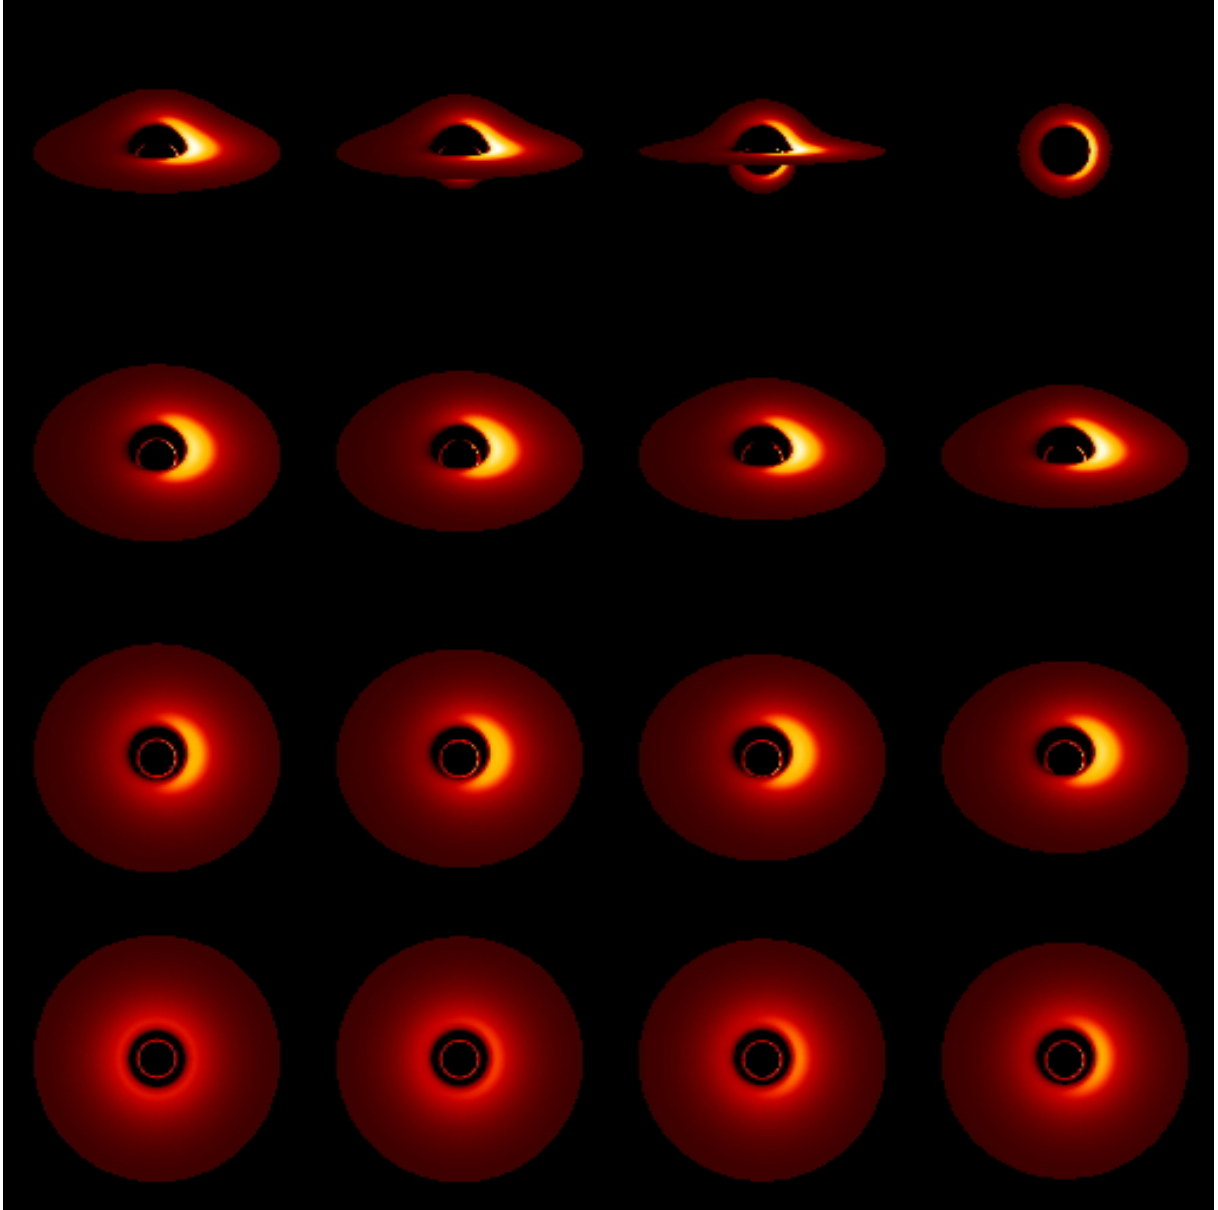
\includegraphics[width=0.5\linewidth]{Images/marck_1989}
	\caption{Imagen de un agujero negro para distintos ángulos. J.A. Marck (1989).}
	\label{fig:marck1989}
\end{figure}

\subsubsection{Imagen de un agujero negro de Schwarzschild desnudo}

\subsubsection{Imagen de un agujero negro de Schwarzschild cubierto}

Antes de comenzar a trabajar, es conveniente introducir las llamadas unidades naturales, definidas por

\begin{equation}
G = \hbar = c = 1.
\label{ec:unidades naturales}
\end{equation}


\section{Solución de Schwarzschild}

La solución de Schwarzschild se considera la solución más sencilla y útil de las ecuaciones de campo de Einstein. Esta solución corresponde a la descripción de un sistema con las siguientes propiedades: \cite{Luminet_1979} \cite{Amarilla_2012} \cite{Amarilla_2018}

\begin{enumerate}
\item Tiene simetría esférica.
\item Es estática e invariante bajo inversión temporal
\item Está en el vacío. 
\end{enumerate}

La solución de Schwarzschild está dado por el intervalo

\begin{equation}
\text{d}s^{2} = -\left( 1 - \dfrac{2M}{r} \right)\text{d}t^{2} + \left( 1 - \dfrac{2M}{r} \right)^{-1}\text{d}r^{2}
+ r^{2}\text{d}\theta^{2} + r^{2}\sin^{2}\theta\text{d}\varphi^{2}
\label{ec:intervalo Schwarzschild}
\end{equation}

La solución de Schwarzschild es particularmente especial debido al llamado teorema de Birkhoff. G. D. Birkhoff demostró en 1923 que cualquier solución con simetría esférica a las ecuaciones de Einstein en el vacío $ \left( \tensor{T}{_\mu_\nu} = 0 \right) $ debe ser estática y asintóticamente plana. La solución de Schwarzschild ha sido construida exigiendo que el espacio–tiempo sea esféricamente simétrico, estático y en el vacío; por lo que la solución no sólo es simple, sino también única.

\subsection{Cantidades conservadas en Schwarzschild}

\subsection{Órbitas de partículas libres en Schwarzschild}

\subsection{Coordenadas celestes}

\section{Solución de Kerr}

El espacio-tiempo alrededor de un agujero negro que rota con masa $M$ y momento angular $J$ puede ser descrito con el intervalo (con $c$ = $G$ = 1)

\begin{equation}
ds^{2} = -\left( 1 - \dfrac{2Mr}{\rho^{2}} \right)dt^{2} - \dfrac{4Mar\sin^{2}\theta}{\rho^{2}}d\varphi dt + \dfrac{\rho^{2}}{\Delta}dr^{2} + \rho^{2}d\theta^{2} + \left( r^{2} + a^{2} + \dfrac{2Mra^{2}\sin^{2}\theta}{\rho^{2}} \right) \sin^{2}\theta d\varphi^{2},
\label{ec:intervalo Kerr}
\end{equation}

donde

\begin{equation}
a \equiv \dfrac{J}{M}, \quad \rho^{2} \equiv r^{2} + a^{2}\cos^{2}\theta, \quad \Delta \equiv r^{2} - 2Mr + a^{2}. 
\label{ec:definiciones en Kerr}
\end{equation}

La métrica definida en \eqref{ec:intervalo Kerr} es una solución exacta a las ecuaciones de campo de Einstein en el vacío, es decir, $G_{\mu\nu} = 0$. Las coordenadas $(t, r, \theta, \varphi)$ usadas en \eqref{ec:intervalo Kerr} se llaman coordenadas de Boyer-Lindquist. 

\subsection{Cantidades conservadas en Kerr}


\subsection{Órbitas de partículas libres en Kerr}

\bibliographystyle{plain}
\bibliography{bib.bib}
	
\end{document}